%
% \documentclass[a4paper, 12pt, times]{article}
% \usepackage{graphicx}
% \usepackage{amsmath}
% \usepackage{amssymb}
% \usepackage{natbib}
% \usepackage{fancyhdr}
% \usepackage{titlesec}
% \usepackage[font=footnotesize]{caption}
%
% \oddsidemargin 0mm \topmargin 0mm \textheight 247mm \textwidth 160mm
% \voffset 0mm \hoffset 0mm \headheight = 0mm \headsep = 0mm
% \pagestyle{fancy}
% \pagenumbering{arabic}
% \fancyhead{}
% \cfoot{\footnotesize ${\rm VIII^{th}}$ Int. Symp. on Stratified Flows, San Diego, USA, Aug. 29 - Sept. 1, 2016}
% \rfoot{\footnotesize \thepage}
% \renewcommand{\headrulewidth}{0pt}
% \setcounter{secnumdepth}{2}
%
% \newfont{\tit}{ptmb at 14pt}      %% Commands to use required fonts.
% \newfont{\auth}{ptmr at 12pt}
% \newfont{\sect}{ptmb at 12pt}
% \newfont{\subsect}{ptmb at 11pt}
%
% \titleformat{\section}{\sect}{\thesection}{1em}{}
% \titleformat{\subsection}{\subsect}{\thesubsection}{1em}{}
%
% \newcommand{\acknowledgements}[0]{\vspace{16pt} \noindent {\sect Acknowledgements} \vspace{10pt}\\}
% \newcommand{\references}[0]{\vspace{16pt} \noindent {\sect References} \vspace{10pt}\\}
% \renewcommand{\abstract}[0]{\noindent {\sect Abstract} \vspace{5pt}\\}

%%%%%%%%%%%%%%%%%%%%%%%%%%%%%%%%%%%%%%%%%%%%%%%%%%%%%%%%

% \newcommand{\R}{\mathcal{R}}
%
% \newcommand{\eps}{\varepsilon}
% \newcommand{\epsK}{\varepsilon_{\!\scriptscriptstyle K}}
% \newcommand{\epsA}{\varepsilon_{\!\scriptscriptstyle A}}
%
% \newcommand{\pathfigures}{/fsnet/project/coriolis/2016/16MILESTONE/figure}
% % \newcommand{\pathfigures}{/home/pierre/16MILESTONE/Figures}
%
% %%%%%%%%%%%%%%%%%%%%%%%%%%%%%%%%%%%%%%%%%%%%%%%%%%%%%%%%
%
% \begin{document}
% \begin{center}
%
% {\tit First report of the MILESTONE experiment: strongly stratified turbulence
% and mixing efficiency in the Coriolis platform}\\ %% Title
%
% \vspace{10pt}
%
% {\auth \underline{Antoine Campagne}$^{1}$, Henrik Alfredsson$^{2}$, R\'emi Chassagne$^{1}$, Diane
% Micard$^{3}$, Nicolas Mordant$^{1}$, Antonio Segalini$^{2}$, Joel
% Sommeria$^{1}$, Samuel Viboud$^{1}$, Ashwin Vishnu Mohanan$^{2}$,\\ Erik
% Lindborg$^{2}$ and Pierre Augier$^{1}$}\\ %%Authors
%
%
% \vspace{10pt}
%
% %%Addresses & emails
% {$^{1}$LEGI, Universit\'{e} Grenoble Alpes, CNRS, France}\\
% {$^{2}$Royal Institute of Technology (KTH), Department of Mechanics, Stockholm, Sweden}\\
% {$^{3}$LMFA, \'Ecole Centrale de Lyon, France}\\
%
% Antoine.Campagne@univ-grenoble-alpes.fr
% \end{center}
%
% \abstract
%
% \noindent Strongly stratified turbulence is a possible interpretation of oceanic and
% atmospheric measurements. However, this regime has never been produced in a
% laboratory experiment because of the two conditions of very small horizontal
% Froude number $F_h$ and large buoyancy Reynolds number $\R$ which require a verily large experimental facility. We
% present a new attempt to study strongly stratified turbulence experimentally in
% the Coriolis platform. The flow is forced by a slow periodic movement of an
% array of six vertical cylinders of 25\ cm diameter with a mesh of 75\ cm.
% %
% Five cameras are used for 3D-2C scanned horizontal particles image velocimetry
% (PIV) and stereo 2D vertical PIV.  Five density-temperature probes are used to
% measure vertical and horizontal profiles and signals at fixed positions.
% %
% The first preliminary results indicate that we manage to produce strongly
% stratified turbulence at very small $F_h$ and large $\R$ in a laboratory
% experiment.


\section{Introduction} 

\noindent
Our understanding of the dynamics of turbulence strongly influenced by a stable
density stratification has been deeply changed at the beginning of the 21st
century.
%
Studies based on large-resolution numerical simulations have shown that there
is a strongly stratified regime associated with a downscale energy cascade
\citep[]{RileyDeBruynKops2003, Lindborg2006}.
%
It has been understood that the stratified turbulence is characterised by two
important non-dimensional numbers and that the regime called ``strongly
stratified turbulence'' is obtained only for very small horizontal Froude
number and large buoyancy Reynolds number \citep[]{Billant2001,
BrethouwerBillantLindborg2007},
\begin{equation}
 F_h = \frac{\epsK}{N U^2} \ll 1,\quad \R = \frac{\epsK}{\nu N^2} > 10,
\label{eq:FhR}
\end{equation}
where $\epsK$ is the kinetic energy dissipation, $N$ the
Brunt-V\"{a}iss\"{a}l\"{a} frequency, $U$ the root-mean-square horizontal
velocity and $\nu$ the kinematic viscosity.
%
\cite{RileyLindborg2008} showed that strongly stratified turbulence is a
possible interpretation for some geophysical turbulent measurements.

\noindent In a laboratory experiment, it is very difficult to fulfill the two conditions $F_h \ll 1$ and $\R > 10$ at the same time, since this requires very large
facilities.
%
Most of stratified flows studied experimentally
correspond to a regime very different than strongly stratified geophysical
flows \citep[see for example][]{PraudFinchamSommeria2005,
AugierBillantNegrettiChomaz2013, AugierBillantChomaz2015}.
%
\cite{BrethouwerLindborg2009} and \cite{Maffioli2016} investigated numerically
the mixing produced by strongly stratified turbulence and showed that at very
small horizontal Froude number ($F_h < 0.03$) and large buoyancy Reynolds
number, the mixing efficiency tends to be independent of these parameters with
a mixing coefficient $\Gamma = \epsA/\epsK$ of the order of 0.35, where $\epsA$
and $\epsK$ are the dissipation rates of available potential energy and kinetic
energy, respectively. This value is nearly twice larger that the canonical
value 0.2 used for mixing parametrization in oceanic models. Moreover, the
effect of rotation on mixing efficiency of strongly stratified
turbulence has to be investigated.

\noindent We present the first report of the EuHIT project experiment (called
MILESTONE) dedicated to better understand these issues by careful measurements
of strongly stratified turbulence in a large-scale experiment in the Coriolis
platform.


\section{Experimental setup}

\begin{figure}[htb]
\centerline{
\includegraphics[width=10cm]{Figures/scheme_exp_grid_MILESTONE_Euhit.pdf}}
\vspace{5mm}
\centerline{
\includegraphics[width=0.45\textwidth]{Figures/GOPR1453.pdf}
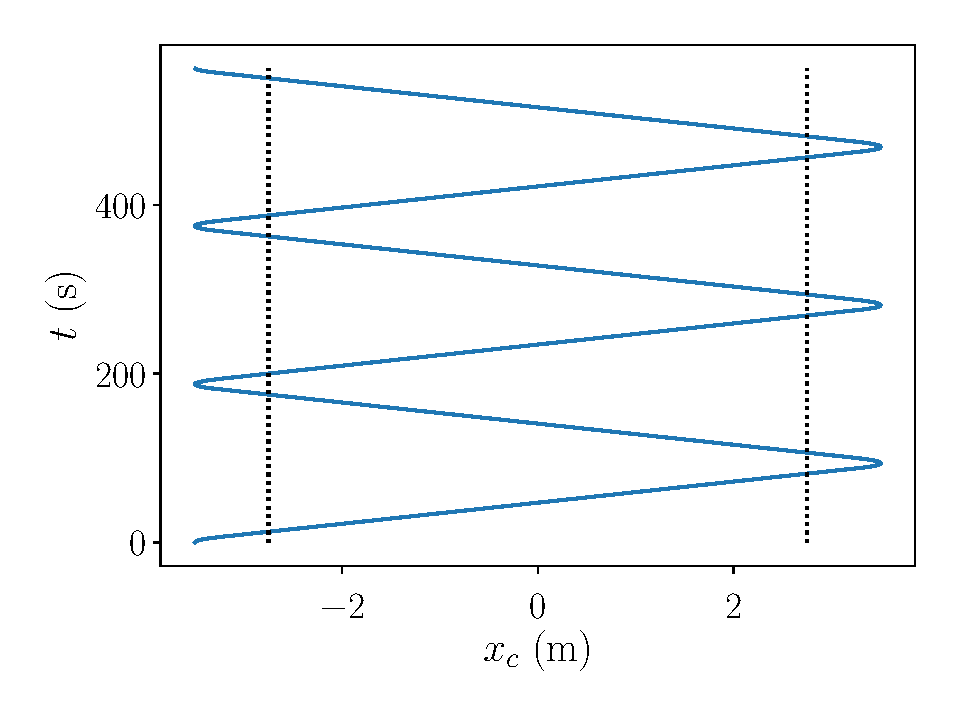
\includegraphics[width=0.45\textwidth]{Figures/fig_movement_carriage.pdf}}
\caption{Top: scheme of the experimental setup (see text for
description). Bottom left: photography of the experiment. Two of our cameras
are visible (highlighted in red), the third one being below the window
highlighted by the black rectangle. Three of our five probes are highlighted in
blue, $P_c$ is embarked on the carriage and $P_p^1$ and $P_p^2$ are attached to
profilers. The vertical PIV field of view and its associated cameras are not
visible in the photo. Bottom right: chronogram of the position of the carriage
$x_c(t)$.}
\label{fig:exp}
\end{figure}

\begin{figure}
\centerline{\includegraphics[]{Figures/fig_profiles.pdf}}
\vspace{-2mm}
\caption{Left: density profiles for $N=0.8$ rad/s and $U_c = 6$ cm/s. Right:
variations of density with respect to the profile at rest
$\Delta\rho=\rho-\rho(t/T=-0.13)$.}
\label{fig_profiles}
\end{figure}

\subsection{Overview of the experiment}
\noindent The experimental setup, installed in the large Coriolis platform, is
presented in figure~\ref{fig:exp}: a tank with a rectangle base of
9$\times$6~m$^2$ area is filled with an approximately linear salt
stratification of $81$~cm depth. The flow is generated with an oscillating
comb consisting of 6 vertical cylinders of $25$~cm diameter attached to a
carriage with a mesh of $M=75$~cm. We impose on the carriage the following
periodic motion of period $T$ (see figure~\ref{fig:ken} for a chronogram of its
position $x_c$): it accelerates with a constant acceleration over 25~cm to a
velocity $U_c$, travels at the uniform speed a distance of 550~cm and
decelerates with a constant deceleration over 25~cm.  It them comes back to its
initial position with the opposite movement and immediately restarts this
cycle. In the following, we use cartesian coordinates with the origin
centered with respect to the vertical walls and at the bottom of the tank. The
vertical coordinate is given by $z$ and the horizontal coordinate along the
direction of displacement of the carriage by $x$ such that $(x,y,z)$ form right
handed coordinates.

\noindent We performed a large number of experiments varying the velocity $U_c$
of the carriage and the linear stratification characterized by the
Brunt-V\"aiss\"al\"a frequency
\begin{equation}
 N =  \sqrt{-\frac{g}{\langle\rho\rangle_z}~\frac{\partial \rho}{\partial z}},
\end{equation}
where $g$ denotes the gravitational acceleration, $\rho$ the volumetric mass
density of the fluid and $\langle\cdot\rangle_z$ the vertical average. In
practice, $N$ is evaluated from the density profile $\rho(z)$ measured at rest,
the slope $\partial\rho/\partial z$ being computed by a linear fit over
$\rho(z)$ on 20~cm around the mid-height of water. A single experiment can be
characterized by two dimensionless parameters based on the forcing control
parameters, a horizontal Froude number and a buoyancy Reynolds number, defined
as
\begin{equation}
 F_{hc} = \frac{U_c}{NM},\quad \R_c = \frac{{U_c}^3}{\nu N^2 M}.
\label{eq:c}
\end{equation}


\begin{table}
\centering
\begin{tabular}{lcccccc}
    \toprule
    &   $Uc$ &  $D_c$ &  $N$  &  $F_{hc}$ &  $Re_c$ &   $\R_c$  \\
    & (cm/s) &   (cm) &(rad/s)&           &         &           \\
    \midrule

 M16-18 &   2 &  25 &  0.76 &  0.100 &   5000 &     50 \\
 M16-21 &   8 &  25 &  0.76 &  0.400 &  20000 &   3200 \\
 M16-22 &   4 &  25 &  0.77 &  0.200 &  10000 &    400 \\
 M16-24 &  16 &  25 &  0.75 &  0.800 &  40000 &  25600 \\
 M16-32 &   2 &  25 &  0.58 &  0.143 &   5000 &    102 \\
 M16-33 &   2 &  25 &  0.58 &  0.143 &   5000 &    102 \\
 M16-34 &   4 &  25 &  0.57 &  0.286 &  10000 &    816 \\
 M16-35 &   4 &  25 &  0.57 &  0.286 &  10000 &    816 \\
 M16-64 &   2 &  25 &  0.74 &  0.100 &   5000 &     50 \\
 M16-65 &   2 &  25 &  0.74 &  0.100 &   5000 &     50 \\
 M16-66 &   4 &  25 &  0.75 &  0.200 &  10000 &    400 \\
 M16-68 &   6 &  25 &  0.76 &  0.300 &  15000 &   1350 \\
 M16-69 &   6 &  25 &  0.74 &  0.300 &  15000 &   1350 \\
 M16-70 &   8 &  25 &  0.76 &  0.400 &  20000 &   3200 \\
 M16-71 &  12 &  25 &  0.70 &  0.600 &  30000 &  10800 \\
 M16-72 &  16 &  25 &  0.68 &  0.800 &  40000 &  25600 \\
 M16-73 &  16 &  25 &  0.56 &  0.800 &  40000 &  25600 \\
 M17-11 &  16 &  25 &  0.55 &  1.164 &  40000 &  54162 \\
 M17-17 &   4 &  50 &  0.55 &  0.145 &  20000 &    423 \\
 M17-18 &   8 &  50 &  0.55 &  0.291 &  40000 &   3385 \\
 M17-19 &   2 &  50 &  0.55 &  0.073 &  10000 &     53 \\
 M17-20 &   2 &  50 &  0.55 &  0.073 &  10000 &     53 \\
 M17-21 &  12 &  50 &  0.55 &  0.436 &  60000 &  11425 \\
 M17-22 &  12 &  50 &  0.55 &  0.436 &  60000 &  11425 \\
 M17-23 &  16 &  50 &  0.55 &  0.582 &  80000 &  27081 \\
 M17-34 &   2 &  25 &  0.55 &  0.145 &   5000 &    106 \\
 M17-35 &   1 &  25 &  0.55 &  0.073 &   2500 &     13 \\
 M17-36 &   4 &  25 &  0.55 &  0.291 &  10000 &    846 \\
 M17-37 &   8 &  25 &  0.55 &  0.582 &  20000 &   6770 \\
 M17-39 &  12 &  25 &  0.55 &  0.873 &  30000 &  22850 \\
 M17-40 &  12 &  25 &  0.55 &  0.873 &  30000 &  22850 \\
 M17-41 &  16 &  25 &  0.55 &  1.164 &  40000 &  54162 \\
 M17-42 &  24 &  25 &  0.55 &  1.745 &  60000 &  182797 \\
 M17-43 &  24 &  25 &  0.55 &  1.745 &  60000 &  182797 \\
 \bottomrule
\end{tabular}
\caption{\label{table:exp} Experiments used for this study.}
\end{table}


\noindent Table~\ref{table} presents the parameters spanned with the
experiments performed without rotation. Thanks to the large dimensions of our
facility, we obtain small to moderate Froude numbers $F_{hc}\in[0.03,~ 0.53]$
and small to large buoyancy Reynolds numbers $\R_c\in[15,~ 34133]$.
%
\noindent Analysis on scaling laws with respect to $F_{hc}$ and $\mathcal{R}_c$
is of course needed for a careful understanding of the flows. However, as this
project is at its earliest stage, a thorough analysis has not yet been
done. For the sake of simplicity, we only present here preliminary results from
the case for $F_{hc} = 0.1$ and $\mathcal{R}_c=450$ (highlighted by bold font
in table~\ref{table}).

\subsection{Measurements}
\noindent This experiment benefits from a well-furnished instrumentation which is
described in the following.

\paragraph{Density measurements}
Five calibrated conductimetric probes $P_i^j$ measure the volumetric
mass density (see figure~\ref{fig:exp}).
%
The probe $P_c$ is embarked on the carriage at the position $(x_c(t)+0.48$,
0.71, 0.395)~m. Since the position of this probe breaks the symetry with
respect to the $x$-axis, its signal has to be separated into two phases. When
the probe is downstream, the measurement can be interpreted as the
statistically stationary signal of a forced turbulence. When the probe is
upstream, we can suppose that the probe is not affected by the
cylinders. The measurement can then be interpreted as the signal of the
decaying turbulence that has been generated during the previous phase.

\noindent The probes $P_f^1$ and $P_f^2$ are respectively placed near the bottom
$(2.73, 2.18, 0.025)$~m and near the surface $(2.73, 2.18, 0.785)$~m in order
to measure the time evolution of the mixed layers.
%
\noindent Finally, the probes $P_p^1$ and $P_p^2$ are fixed on well controlled
vertical profilers at positions $(-1.01, 2.24, z_p(t))$ and
$(1.66, 2.14, z_p(t))$, respectively. The short time response of the probes and
the rapidity of the profilers allow us to get well resolved vertical density
profiles over 70~cm height on a time of $8$~s. Figure~\ref{fig_profiles}
represents three density profiles during an experiment consisting of 7 periods
of oscillation of the carriage. The blue line corresponds to the background
profile with fluid at rest. It shows a well defined linear dependence below  $z=65$~cm
and a mixed layer near the surface. The expected mixed layer at the bottom is not present here since the probes does not approach enough the bottom of the
tank.
%
Profiles at later times show density fluctuations with respect to the
background profile of the order of 1~kg/m$^3$ which corresponds to a
typical vertical displacement of isopycnals of 1~cm. In the profile
for $t/T = 9.56$ (yellow curves), we see that part of these fluctuations persist a long
time after the carriage stops. Importantly, we see that we can easily measure
the density variation in time at the surface that will allow us to compute
the mixing efficiency for every experiment.


\paragraph{PIV measurements}
 We measure vertical and horizontal velocity fields using two PIV
systems. The vertical measurement domain is a $0.45 \times 0.45$~m$^2$ vertical
square with a resolution of 5~mm centered at the position
$(1.88, 2.20, 0.35)$~m. We acquire up to 1300 images per period of oscillation
$T$ with a $1024^2$ pixel camera.

\noindent Horizontal fields are measured with 2D scanned PIV system with a
rapid vertically oscillating horizontal laser sheet. The vertical position of
the laser sheet is given by a staircase profile with up to 11 levels on a time
less than 100~ms. Oscillation of the laser sheet is achieved by an
oscillating mirror placed 6~m from the region of interest. Half of the depth can be scanned with quasi-horizontal laser sheets, with the angle of the
laser sheet with respect to the horizontal being less than $1.5^{\circ}$. In
practice, two sets of measurement are done: one with a small scan amplitude
(five planes with $z\in[0.483,~0.514]$~m) in order to resolve small vertical
scale structures. The second set is performed with a large scan amplitude
(typically eight planes with $z\in[0.252,~,0.554]$~m) that provides more
vertically decorrelated fields.
%
Images are acquired by three $2560\times2160$ pixel cameras synchronized with
the oscillating mirror, each camera looking on three different regions of
interest (see figure~\ref{fig:exp}). Two of them are centered at $y=0$ with a
large and a small field. The larger field ($2.2\times2.5$~m$^2$) is acquired
from the top through the water surface and the small field
($1.18\times0.53$~m$^2$) through a glass from the bottom of the tank. The third
view ($1.3\times1.0 $~m$^2$) is taken at the vicinity of a side wall. We
acquire up to 1300 images per vertical level of the laser sheet and per period
of the movement of the cylinders.

\noindent Acquisition of images begins after one period of oscillation of the
carriage and ends one period after the carriage stops. The forcing consists of
3 periods of oscillation for the small amplitude scan case and 12 periods for
large scan amplitude case.

\noindent Figure~\ref{fig:field} shows instantaneous horizontal and vertical velocity
fields for $t/T = [$1.31, 1.5, 1.68$]$. 
%
The resolution is equal to $5.3$~mm for the vertical cross-section and $2.3$~cm
for the horizontal cross-section.
%
Note that, as the turbulence is inhomogeneous and positions of measurement of
horizontal and vertical fields are different, these former fields cannot be
mutually described. Just after the carriage quit the field of view of the
camera ($t/T=1.31$), horizontal field exhibits energetic vortices of typical
sizes of $M$. At larger times, we observe the persistence of large horizontal
scale structures. Furthermore, vertical fields show strongly horizontally
elongated structures, which is a robust feature of turbulence in stratified
fluids.

\begin{figure}[htb]
\centerline{
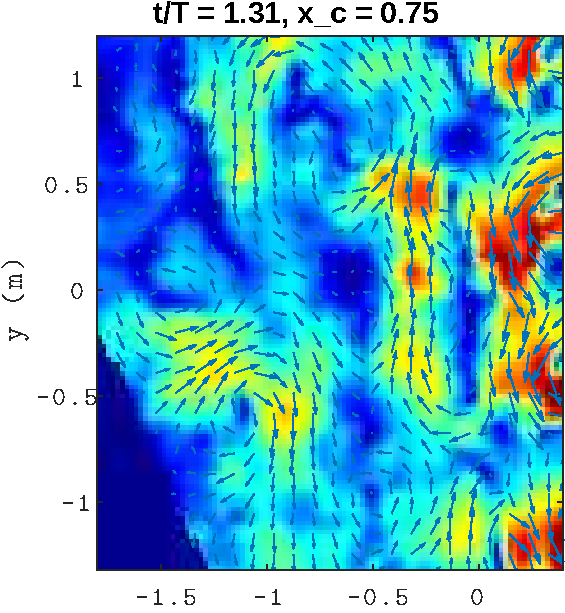
\includegraphics[width=4.14cm]{paper_05_milestone_issf/Figures/exp21/vh_400.pdf}
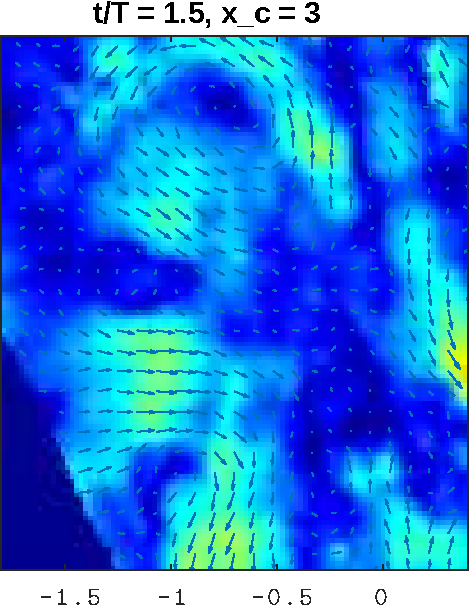
\includegraphics[width=3.44cm]{paper_05_milestone_issf/Figures/exp21/vh_655.pdf}
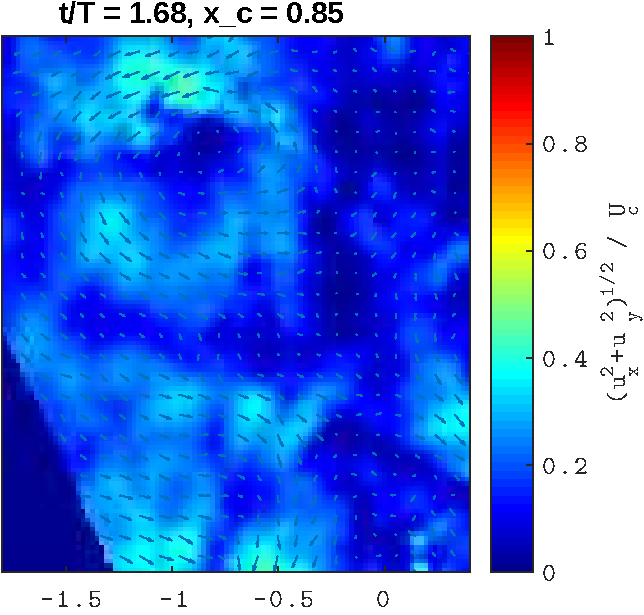
\includegraphics[width=4.72cm]{paper_05_milestone_issf/Figures/exp21/vh_890.pdf}}
\vspace{0mm}
\centerline{
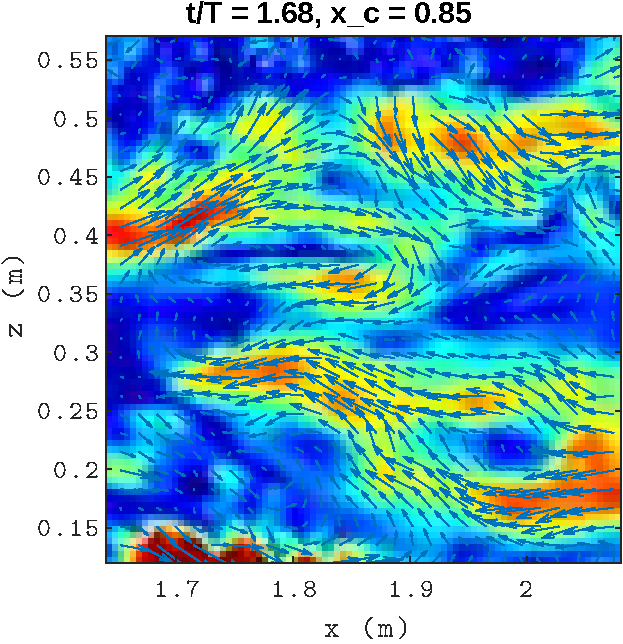
\includegraphics[width=4.16cm]{paper_05_milestone_issf/Figures/exp21/vv_890.pdf}
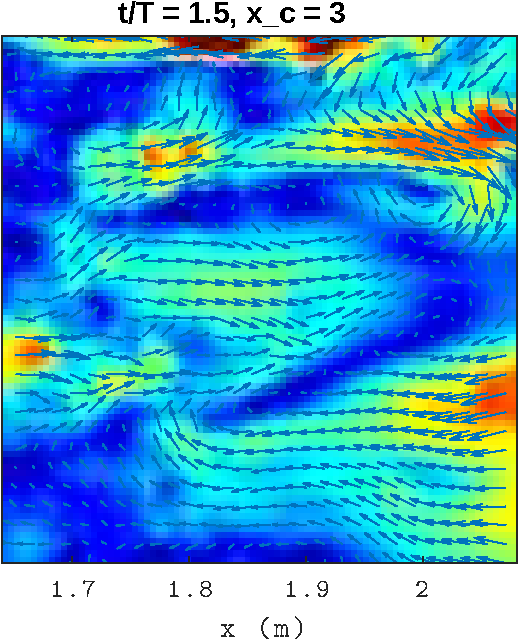
\includegraphics[width=3.48cm]{paper_05_milestone_issf/Figures/exp21/vv_655.pdf}
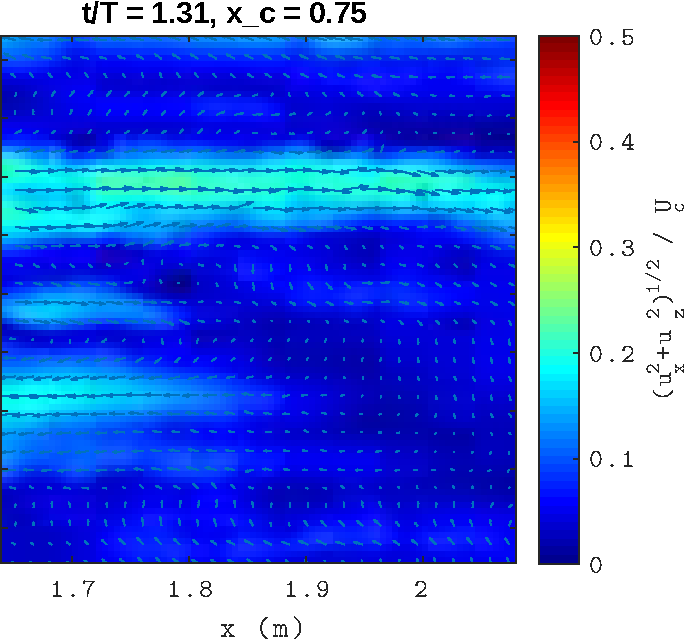
\includegraphics[width=4.63cm]{paper_05_milestone_issf/Figures/exp21/vv_400.pdf}
}
\vspace{-2mm}
\caption{Instantaneous horizontal large fields (top, $z=40$~cm) and vertical
fields (bottom) for $t/T = [1.31,~1.5,~1.68]$, $F_{hc} = 0.1$ and
$\mathcal{R}_c=450$. Background colors indicate the norm of the 2D field
normalized by $U_c$, which is $(u_x^2 + u_y^2)/U_c$ and $(u_x^2 + u_z^2)/U_c$,
respectively.}
\label{fig:field}
\end{figure}


\section{Preliminary results for $F_{hc} = 0.1$ and $\mathcal{R}_c=450$}

With this setup, energy is injected locally by an oscillating comb of
cylinders. Turbulence in a given region of interest is therefore inhomogeneous
and unstationary. Evolution of kinetic energy with time is then an important
feature of this flow. Figure~\ref{fig:ken} represents the normalized horizontal
kinetic energy $\langle u_x^2 + u_y^2 \rangle/2U_c^2$ as a function of the
fractional part of normalized time $\{t/T\}$ for 5 particular periods, with
$\langle\cdot\rangle$ denoting 3D spatial average. Kinetic energy is computed
from large horizontal PIV fields for each time when the carriage does not
appear in the field of view of the camera. The carriage is stopped at the end
of the 12th period. The flow undergoes successive turbulent decays. The energy
injects is of the order of $U^2 \simeq 0.08 U_c^2$.
%
We estimate the mean kinetic energy dissipation rate to
$\epsK \simeq 2 \times 10^{-2} U_c^3/M$ by computing the time average of
$-\partial\langle u_x^2+u_y^2\rangle/\partial t$ over $0.3 < \{t/T\} < 0.35$.


\begin{figure}[htb]
\centerline{
\includegraphics[width=9.cm]{paper_05_milestone_issf/Figures/exp28/ken_fct_t_T_exp28.pdf}}
\vspace{-2mm}
\caption{Spatial average of normalized horizontal kinetic energy
$\langle u_x^2 + u_y^2\rangle/2U_c^2$ as a function of the fractional part of
the normalized time $\{t/T\}$ for different periods of measurement and for
$F_{hc} = 0.1$ and $\mathcal{R}_c=450$. Times where no data appears corresponds
to those when the carriage is in the field of view and hides a part of the
field of view. The gray line represents the position of the carriage $x_c$ and
the three red circles mark the times chosen for the figure~\ref{fig:field}. The
pair of symbols $\vartriangleleft-\vartriangleright$ delimits the ranges of
time where the carriage appears in the field of view.}
\label{fig:ken}
\end{figure}

\noindent We now characterize the distribution of energy among scales by second-order
structure function, defined as
\begin{eqnarray}
S_h(r) = (S_{xx} + S_{yy} + S_{xy} + S_{yx})/2,\\
\text{with} \quad S_{ij} = \langle\overline{(u_i({\bf x}+r{\bf e}_j)-u_i({\bf x}))^2}\rangle,
\end{eqnarray}
and $\overline{\cdot}$ time average when the carriage is moving. For a
developed turbulence, and for scales larger than the dissipative scale and
lower than injection scale, we expect
$S_h(r) = C (\varepsilon r)^{2/3} = C' (rU_c^3/M)^{2/3}$, with $C$ a coefficient
approximately equal to 6 \citep[see figure 15 in][]{AugierBillantChomaz2015}.
\begin{figure}[htb]
\centerline{
\includegraphics[height=7.5cm]{paper_05_milestone_issf/Figures/exp28/normalized_S2_exp28.pdf}}
\vspace{-2mm}
\caption{Normalized second-order structure $S_h$ function as a function of
$r/M$ for $F_{hc} = 0.1$ and $\mathcal{R}_c=450$.}
\label{fig:S2}
\end{figure}
Figure~\ref{fig:S2} represents normalized second-order structure function
computed from large horizontal fields for a 12 periods forcing
experiment. Interestingly, the curve exhibits a plateau corresponding to a
$r^{2/3}$ scaling law on half a decade at a value going from $0.4$ at
$\{t/T\} = 0.31$ to $0.2$ at $\{t/T\} = 0.31$. Supposing that this range
corresponds to an inertial range, we evaluate a surrogate of the mean
dissipation rate at $\epsK \sim 0.01 U_c^3/M$. This order of magnitude is
consistent with the previous estimation by direct computation of the energy
decay.

\noindent By extrapolation of the energy dissipation rate and energy injected
at the vicinity of the carriage, we define surrogates of the turbulent
horizontal Froude and buoyancy Reynolds numbers based on the measured flow as
\begin{equation}
F_{he} \simeq \frac{\epsK}{N U^2} \simeq 0.25 F_{hc},\quad 
\R_e \simeq \frac{\epsK}{\nu N^2} \simeq 2\times10^{-2} \R_c.
\label{eq:e}
\end{equation}
For this case for $F_{hc} = 0.1$ and $\mathcal{R}_c=450$, we find
$F_{he} \simeq 0.02$ and $\mathcal{R}_e \simeq 9$. These orders of magnitude
correspond to flows for which a downscale energy cascade and horizontal spectra
with a -5/3 scaling law have been observed numerically
\citep[]{BrethouwerBillantLindborg2007, AugierBillantChomaz2015}.
%
This strongly indicates that the $r^{2/3}$ scaling law for $S_h$ is indeed
related to strongly stratified turbulence.

\noindent The values of these dimensionless parameters given in table~\ref{table} for the
other cases show that we were able with this experiment setup to span very
interesting ranges of parameters, from very strongly stratified
($F_{he} \simeq 0.01$) to weakly stratified ($F_{he} \simeq 0.1$) and from
small to large buoyancy Reynolds numbers.
%
Although the analysis of the data is still at a very preliminary stage, the
reached values of the turbulent numbers $F_{he}$ and $\R_e$ will enable us to
address the question of mixing efficiency in the regime relevant of the ocean
dynamics.

\section*{Acknowledgements}

This project has received funding from the foundation Simone et Cino Del Duca de
l'Institut de France and the European Research Council (ERC) under the European
Union's Horizon 2020 research and innovation program (grant agreement No
647018-WATU and Euhit consortium).
%
We thank Mile Kusulja, Thomas Valran, Julie Germinario and Gabriel Moreau for
their help to design, build and carry out this experiment.


% \references
% \def\refname{}
% \vspace{-0.9in}
% \bibliographystyle{apalike}
% \bibliography{references}
%
%
% \end{document}
